\documentclass[12pt,a4paper,openany,oneside]{book}

% 格式控制
%------------------------------------------------------------------------------%
%                                                                              %
%   LaTeX Template for Bachlor Thesis of Northwestern Polytechnical University %
%   Environment Config: TeXLive 2017                                           %
%   * XeTeX 3.14159265-2.6-0.99998 (TeX Live 2017/W32TeX)                      %
%   * BibTeX 0.99d (TeX Live 2017/W32TeX)                                      %
%   Version: 1.5.0.0426                                                        %
%                                                                              %
%------------------------------------------------------------------------------%
%   Copyright by NWPU Metaphysics Office, GPLv3-LICENSE                        %
%------------------------------------------------------------------------------%


%---------------------------------纸张大小设置---------------------------------%
\usepackage{geometry}
% 普通A4格式缩进
\geometry{left=3.18cm,right=3.18cm,top=1in,bottom=1.5in}  %页边距
% 论文标准缩进
% \geometry{left=1.25in,right=1.25in,top=1in,bottom=1.5in}
%------------------------------------------------------------------------------%


%----------------------------------必要库支持----------------------------------%
\usepackage{xcolor}
\usepackage{tikz}
\usepackage{layouts}
\usepackage[numbers,sort&compress]{natbib}
\usepackage{clrscode}
\usepackage{gensymb}
\usepackage[final]{pdfpages}
%------------------------------------------------------------------------------%
\usepackage{float}%图片排版
\usepackage{subfig}%m图片排版
\usepackage{afterpage}
\newcommand\myemptypage{
    \null
    \thispagestyle{empty}
    \newpage
    }
% \usepackage{mathptmx}
%--------------------------------设置标题与目录--------------------------------%
\usepackage[sf]{titlesec}
\usepackage{titletoc}



%------------------------------------------------------------------------------%


%--------------------------------添加书签超链接--------------------------------%
\usepackage[unicode=true,colorlinks=false,pdfborder={0 0 0}]{hyperref}
% 在此处修改打开文件操作
\hypersetup{
    bookmarks=true,         % show bookmarks bar?
    pdftoolbar=true,        % show Acrobat’s toolbar?
    pdfmenubar=true,        % show Acrobat’s menu?
    pdffitwindow=true,      % window fit to page when opened
    pdfstartview={FitH},    % fits the width of the page to the window
    pdfnewwindow=true,      % links in new PDF window
}
% 在此处添加文章基础信息
\hypersetup{
    pdftitle={title},
    pdfauthor={author},
    pdfsubject={subject},
    pdfcreator={creator},
    pdfproducer={producer},
    pdfkeywords={key1  key2  key3}
}
%------------------------------------------------------------------------------%


%---------------------------------设置字体大小---------------------------------%
\usepackage{type1cm}
% 字号与行距,统一前缀s(a.k.a size)
\newcommand{\sChuhao}{\fontsize{42pt}{63pt}\selectfont}                 % 初号, 1.5倍
\newcommand{\sYihao}{\fontsize{26pt}{36pt}\selectfont}                  % 一号, 1.4倍
\newcommand{\sErhao}{\fontsize{22pt}{28pt}\selectfont}                  % 二号, 1.25倍
\newcommand{\sXiaoer}{\fontsize{18pt}{18pt}\selectfont}                 % 小二, 单倍
\newcommand{\sSanhao}{\fontsize{16pt}{24pt}\selectfont}                 % 三号, 1.5倍
\newcommand{\sXiaosan}{\fontsize{15pt}{22pt}\selectfont}                % 小三, 1.5倍
\newcommand{\sSihao}{\fontsize{14pt}{21pt}\selectfont}                  % 四号, 1.5倍
\newcommand{\sHalfXiaosi}{\fontsize{12.5pt}{16.25pt}\selectfont}        % 半小四, 1.25倍
\newcommand{\sLargeHalfXiaosi}{\fontsize{13pt}{19pt}\selectfont}        % 半小四, 1.5倍
\newcommand{\sXiaosi}{\fontsize{12pt}{15.6pt}\selectfont}               % 小四, 1.25倍  常用 
\newcommand{\sXiaosiEng}{\fontsize{12pt}{12.4pt}\selectfont}               % 小四, 1.25倍
\newcommand{\sLargeWuhao}{\fontsize{11pt}{11pt}\selectfont}             % 大五, 单倍
\newcommand{\sWuhao}{\fontsize{10.5pt}{10.5pt}\selectfont}              % 五号, 单倍
\newcommand{\sXiaowu}{\fontsize{9pt}{9pt}\selectfont}                   % 小五, 单倍
%------------------------------------------------------------------------------%

%---------------------------------设置中文字体---------------------------------%
\usepackage{fontspec}
\usepackage[SlantFont,BoldFont,CJKchecksingle]{xeCJK}
\usepackage{CJKnumb}
% 使用 Adobe 字体
\newcommand\defaultSog{SimSun}                      % 宋体, 用于正文
\newcommand\defaultHei{SimHei}                      % 黑体, 用于标题
\newcommand\defaultKai{KaiTi}                       % 楷体, 一般用于强调
\newcommand\defaultFag{FangSong}                    % 仿宋, 一般用于强调
\newcommand\codeFont{Consolas}
%%-----------------------------------------------------------------------------%
\newcommand\defaultEngFont{Times New Roman}                 % 英文文本默认字体    新罗马              
% 设置字体
\defaultfontfeatures{Mapping=tex-text}                      % 启用 TeX Ligatures
\setCJKmainfont[ItalicFont=\defaultKai, BoldFont=\defaultHei]{\defaultSog}
\setCJKsansfont[ItalicFont=\defaultKai, BoldFont=\defaultHei]{\defaultSog}
\setCJKfamilyfont{song}{\defaultSog}                        % 设置 CJK 字体族
\setCJKfamilyfont{hei}{\defaultHei}                         %
\setCJKfamilyfont{kai}{\defaultKai}                         %
\setCJKfamilyfont{fang}{\defaultFag}                        %
\setCJKfamilyfont{eng}{\defaultEngFont}                     %
\setmonofont{\codeFont}                                     %
\setmainfont{\defaultEngFont}                               %
\setCJKfamilyfont{nwpu}{nwpuname}
\newcommand{\fSong}{\CJKfamily{song}}                       % 宋体: fSong
\newcommand{\fHei}{\CJKfamily{hei}}                         % 黑体: fHei
\newcommand{\fKai}{\CJKfamily{kai}}                         % 楷体: fKai
\newcommand{\fFang}{\CJKfamily{fang}}                       % 仿宋: fFang
\newcommand{\fEng}{\CJKfamily{eng}}                         % 英文: fEng
\newcommand{\fNWPU}{\CJKfamily{nwpu}}
%------------------------------------------------------------------------------%


%------------------------------添加插图与表格控制------------------------------%
\usepackage{graphicx}
\usepackage[font=small,labelsep=quad]{caption}
\usepackage{wrapfig}
\usepackage{multirow,makecell}
\usepackage{longtable}
\usepackage{booktabs}
\usepackage{tabularx}
\usepackage{setspace}
\captionsetup[table]{labelfont=bf,textfont=bf}
%------------------------------------------------------------------------------%


%---------------------------------添加列表控制---------------------------------%
\usepackage{enumerate}
\usepackage{enumitem}
%------------------------------------------------------------------------------%


%---------------------------------设置引用格式---------------------------------%
\renewcommand\figureautorefname{图}
\renewcommand\tableautorefname{表}
\renewcommand\equationautorefname{式}
\newcommand\myreference[1]{[\ref{#1}]}
\newcommand\eqrefe[1]{式(\ref{#1})}
% 增加 \ucite 命令使显示的引用为上标形式
\newcommand{\ucite}[1]{$^{\mbox{\scriptsize \cite{#1}}}$}
\renewcommand\arraystretch{1.4}
\renewcommand\theequation{\thechapter-\arabic{equation}}

\renewcommand{\thefigure}{\thechapter-\arabic{figure}}
\renewcommand{\thetable}{\thechapter-\arabic{table}}
%------------------------------------------------------------------------------%


%--------------------------------设置定理类环境--------------------------------%
\usepackage[amsthm,thmmarks]{ntheorem}
\newtheorem{myexample}{例}
\newtheorem{thm}{定理}
%------------------------------------------------------------------------------%


%--------------------------设置中文段落缩进与正文版式--------------------------%
\XeTeXlinebreaklocale "zh"                      % 使用中文的换行风格
\XeTeXlinebreakskip = 0pt plus 1pt              % 调整换行逻辑的弹性大小
\usepackage{indentfirst}                        % 段首空格设置
\setlength{\parindent}{26pt}                    % 段首空格长度
% \setlength{\parskip}{3pt plus 1pt minus 1pt}    % 段落间距  所有段落间距一致
\renewcommand{\baselinestretch}{1.25}           % 行距
%------------------------------------------------------------------------------%


%----------------------------设置段落标题与目录格式----------------------------%
\setcounter{secnumdepth}{3}
\setcounter{tocdepth}{2}

\newcommand\chapterID[1]{第\CJKnumber{#1}章}
\renewcommand{\chaptername}{第\CJKnumber{\thechapter}章}
\renewcommand{\figurename}{图}
\renewcommand{\tablename}{表}
\renewcommand{\bibname}{参考文献}
\renewcommand{\contentsname }{\fHei \sSanhao 目~~~录}
\newcommand{\keywords}[1]{\\ \\ \textbf{关~键~词}:#1}


\titleformat{\chapter}[hang]{\normalfont\sSanhao\filcenter\fHei }
{\sSanhao{\chaptertitlename}}{1em}{\sSanhao} %  三号 黑体
\titleformat{\section}[hang]{\fEng  \sSihao} 
{\sSihao\fHei \thesection}{0.5em}{\fHei}{} % 四号  黑体 
\titleformat{\subsection}[hang]{\fEng  \sLargeHalfXiaosi} %
{\sLargeHalfXiaosi\fHei \thesubsection}{0.5em}{\fHei}{} % 黑体 小四
\titleformat{\subsubsection}[hang]{\fEng }%
{(\arabic{subsubsection})}{0.5em}{\fSong}{}   % 小标题式的subsubsection:(4) 标题

% 缩小正文中各级标题之间的缩进
\titlespacing{\chapter}{0pt}{4pt}{12.25pt}
\titlespacing{\section}{0pt}{0pt}{0em}
\titlespacing{\subsection}{0pt}{0pt}{0em}
\titlespacing{\subsubsection}{0pt}{0pt}{0pt}

% 定义目录中各级标题之间的格式以及缩进
\dottedcontents{section}[1.16cm]{}{1.8em}{5pt}
\dottedcontents{subsection}[2.00cm]{}{2.7em}{5pt}
\dottedcontents{subsubsection}[2.86cm]{}{3.4em}{5pt}
\titlecontents{chapter}[0pt]{\bf  \fSong\vspace{0.5em}}% 宋体
{\contentsmargin{0pt} \bf \fSong \makebox[0pt][l]{\chapterID{\thecontentslabel}}\hspace{3.8em}}%
{\contentsmargin{0pt}\bf \fSong}% 加粗
{\titlerule*[.5pc]{.}\contentspage}[\vspace{0em}]
%------------------------------------------------------------------------------%


%---------------------------------设置页眉页脚---------------------------------%
\usepackage{fancyhdr}
\usepackage{fancyref}
%\addtolength{\headsep}{-0.1cm}          %页眉位置
%\addtolength{\footskip}{-0.1cm}         %页脚位置
\addtolength{\topmargin}{0.5cm}
\newcommand{\makeheadrule}{
    \makebox[0pt][l]{\rule[.7\baselineskip]{\headwidth}{0.8pt}}
    \vskip-.8\baselineskip
}
\makeatletter
\renewcommand{\headrule}{%
    {\if@fancyplain\let\headrulewidth\plainheadrulewidth\fi\makeheadrule}}
\pagestyle{fancyplain}
\fancyhf{}
\fancyfoot[C,C]{\sWuhao~\thepage~}  %页码为单独数字
% 后续文字可以自行修改
\chead{\sSanhao\raisebox{0.04cm}%
    { \fNWPU 西北工业大学} \fSong{{\textbf{本科毕业设计论文} }}} 
%------------------------------------------------------------------------------%


%----------------------------------其他补充设置--------------------------------%
% 重置列表环境的间隔
% \let\orig@Itemize =\itemize
% \let\orig@Enumerate =\enumerate
% \let\orig@Description =\description

% \def\Myspacing{
%     \itemsep=1.5ex \topsep=-0.5ex \partopsep=0pt \parskip=0pt \parsep=0.5ex
% }

% \def\newitemsep{
%     \renewenvironment{itemize}{\orig@Itemize\Myspacing}{\endlist}
%     \renewenvironment{enumerate}{\orig@Enumerate\Myspacing}{\endlist}
%     \renewenvironment{description}{\orig@Description\Myspacing}{\endlist}
% }

% \def\olditemsep{
%     \renewenvironment{itemize}{\orig@Itemize}{\endlist}
%     \renewenvironment{enumerate}{\orig@Enumerate}{\endlist}
%     \renewenvironment{description}{\orig@Description}{\endlist}
% }

% \newitemsep
% 下划线
\newcommand\dlmu@underline[2][5cm]%
{\hskip1pt\underline{\hb@xt@ #1{\hss#2\hss}}\hskip3pt}
\let\coverunderline\dlmu@underline
%------------------------------------------------------------------------------%


%----------------------------------添加代码控制--------------------------------%
\usepackage{listings}
\lstset{
    basicstyle=\footnotesize\ttfamily,
    numbers=left,
    numberstyle=\tiny,
    numbersep=5pt,
    tabsize=4,
    extendedchars=true,
    breaklines=true,
    keywordstyle=\color{blue}\bfseries,
    numberstyle=\color{purple},
    commentstyle=\color[rgb]{0, 0.4, 0}\bfseries,
    stringstyle=\color{violet}\ttfamily\bfseries,
    rulesepcolor=\color{red!20!green!20!blue!20},
    showspaces=false,
    showtabs=false,
    frame=shadowbox,
    framexrightmargin=5pt,
    framexbottommargin=4pt,
    showstringspaces=false,
    escapeinside=`', %逃逸字符(1左面的键),用于显示中文
}
\renewcommand{\lstlistingname}{CODE}
\lstloadlanguages{% Check Dokumentation for further languages, page 12
    Pascal, C++, Java, Ruby, Python, Matlab, R, Haskell
}
%------------------------------------------------------------------------------%

\endinput
% 这是简单的 thesis(book) 的导言区设置,不能单独编译。


% 非格式控制插件
% \usepackage{math-symbols}
\usepackage{plug-ins/math-symbols}
\usepackage{enumitem}

% Longitudinal coefficients
\newcommand\CL{{C_L}}
\newcommand\CLz{{C_{L_0}}}
\newcommand\CLa{{C_{L_\alpha}}}
\newcommand\CLq{{C_{L_q}}}
\newcommand\CLde{{C_{L_{\delta_e}}}}
\newcommand\CD{{C_D}}
\newcommand\CDz{{C_{D_0}}}
\newcommand\CDa{{C_{D_\alpha}}}
\newcommand\CDq{{C_{D_q}}}
\newcommand\CDde{{C_{D_{\delta_e}}}}
\newcommand\Cm{{C_m}}
\newcommand\Cmz{{C_{m_0}}}
\newcommand\Cma{{C_{m_\alpha}}}
\newcommand\Cmq{C_{m_q}}
\newcommand\Cmde{C_{m_{\delta_e}}}
\newcommand\Cmcl{{C_{m_{C_L}}}}

% Lateral coefficients
\newcommand\CY{C_Y}
\newcommand\CYz{C_{Y_0}}
\newcommand\CYb{C_{Y_\beta}}
\newcommand\CYp{C_{Y_p}}
\newcommand\CYr{C_{Y_r}}
\newcommand\CYda{C_{Y_{\delta_a}}}
\newcommand\CYdr{C_{Y_{\delta_r}}}
\newcommand\Cl{C_l}
\newcommand\Clz{C_{l_0}}
\newcommand\Clb{C_{l_\beta}}
\newcommand\Clp{C_{l_p}}
\newcommand\Clr{C_{l_r}}
\newcommand\Clda{C_{l_{\delta_a}}}
\newcommand\Cldr{C_{l_{\delta_r}}}
\newcommand\Cn{C_n}
\newcommand\Cnz{C_{n_0}}
\newcommand\Cnb{C_{n_\beta}}
\newcommand\Cnp{C_{n_p}}
\newcommand\Cnr{C_{n_r}}
\newcommand\Cnda{C_{n_{\delta_a}}}
\newcommand\Cndr{C_{n_{\delta_r}}}

% Controls
\newcommand\da{{\delta_a}}
\newcommand\de{{\delta_e}}
\newcommand\dr{{\delta_r}}
\newcommand\dt{{\delta_t}}

% factor
\newcommand\q{{\frac{1}{2} \rho V^2}}       % 1/2 rho V^2
\newcommand\qs{{\frac{1}{2} \rho V^2 S}}    % 1/2 rho V^2

% others
\newcommand\CW{{C_W}}

\endinput

% 插图目录
\graphicspath{{figures/}}

% 仅用于测试
\usepackage{blindtext}

\title{\textsf{比如我举个例子}}
\author{{\kai 谁知道呢}}
\date{May 20, 20xx}

\begin{document}

\sloppy

\pagenumbering{Roman}

% 封皮
\frontmatter
% 本科毕业设计论文模板
% 封皮
\begin{titlepage}
    \voffset 2.1cm
    \begin{center}
        \begin{center}
            \begin{minipage}[c]{2.64cm}
                \centering
                \resizebox{!}{0.9cm}{ \parbox{0.54cm}{ \begin{tikzpicture}
    \draw[line width=0.10cm] (0, 0) circle (2.0cm);
    % \fill[gray!15] (0, 0) -- (1.3cm,0cm) arc (0:230:1.3cm) -- cycle;
    % \fill[gray!15] (0, 0) -- (1.3cm,0cm) arc (0:-50:1.3cm) -- cycle;
    \foreach \t in {-50, -40, -30, -20, -10, 0, 10, 20, 30, 40, 50, 60, 70, 80, 90, 100, 110, 120, 130, 140, 150, 160, 170, 180, 190, 200, 210, 220, 230}
    {
        \foreach \p/\d in {0/0.01cm, 5/-0.01cm}
        {
            \foreach \r in {1.27cm, 1.17cm, 1.07cm, 0.97cm}
            {
                \fill (\t + \p: \r + \d) circle (0.01cm);
            }
        }
    };
    \draw[line width=0.03cm] (0, 0) circle (1.32cm);
    \fill[white] (0, 0) circle (0.9cm);
    \draw[line width=0.05cm] (0, 0) circle (0.9cm);
    \fill[black] (-0.50, -0.73) .. controls (-0.35, -0.81) ..
        (-0.2, -0.80) .. controls (0.15, -0.70) and (0.20, -0.60) .. 
        (0.35, -0.35) .. controls (0.42, -0.24) and (0.60, -0.26) ..
        (0.60, -0.40) .. controls (0.58, -0.50) and (0.49, -0.50) ..
        (0.45, -0.45) .. controls (0.40, -0.68) and (0.75, -0.70) ..
        (0.90, 0.00) arc (360:250:0.9cm);
    \fill (-0.40, -0.40)--(-1.33, -0.40)--(1.00, 1.10)--cycle;
    \fill (-0.37, -0.43)--(-0.20, -0.80)--(1.01, 1.05)--cycle;
    
    \foreach \x/\txt in {0/N, 1/O, 2/R, 3/T, 4/H, 5/W, 6/E, 7/S, 8/T, 9/E, 10/R, 11/N, 12/~, 13/P, 14/O, 15/L, 16/Y, 17/T, 18/E, 19/C, 20/H, 21/N, 22/I, 23/C, 24/A, 25/L, 26/~, 27/U, 28/N, 29/I, 30/V, 31/E, 32/R, 33/S, 34/I, 35/T, 36/Y}
    {
        \node[scale=0.7, rotate=\x*-6.50-245] at (207+\x*-6.50:1.6cm) {\txt};
    };

    \foreach \x/\txt in {0/西, 1/北, 2/工, 3/业, 4/大, 5/学}
    {
        \node[scale=1.25, rotate=\x*18-50] at (225+\x*18:1.65cm) {\fNWPU\txt};
    };

    \foreach \x/\txt in {0/1, 1/9, 2/3, 3/8}
    {
        \node[scale=1, rotate=\x*18-25] at (\x*18-115:1.1cm) {\bfseries\txt};
    };
\end{tikzpicture}

\endinput
% 这是西北工业大学校徽文件,不能单独编译。 } }
                \end{minipage}
                \hskip 0.8cm
                \begin{minipage}[c]{8cm}
                \fontsize{33}{33}\fNWPU 西北工业大学
            \end{minipage}
        \end{center}
        \vskip 0.7cm
        \sChuhao\fSong {\bfseries 本科毕业设计(论文)}%中文括号
        \vskip 4cm
        {
        \sSanhao\fHei \textbf{ 题~~目}  \hspace{0.2cm}\coverunderline[12.5cm] {\fSong 基于飞行走廊的无人机轨迹规划算法研究}
        }
        \vskip 1.7cm
        {
            \sSihao\fSong 专业名称\coverunderline[5.5cm]{}%自动化
            \vskip 0.9cm
            \sSihao\fSong 学生姓名\coverunderline[5.5cm]{}%冯杰琳
            \vskip 0.9cm
            \sSihao\fSong 指导教师\coverunderline[5.5cm]{}%胡劲文
            \vskip 0.9cm
            \sSihao\fSong 毕业时间\coverunderline[5.5cm]{}%2022年6月
            \vfill
        }
    \end{center}
\end{titlepage}
\fSong \normalsize

\endinput
% 这是封面排版文件,不能单独编译。
%\myemptypage  空一页
\clearpage

\setcounter{page}{1}
\pagenumbering{Roman}
\renewcommand{\baselinestretch}{1.25}

% 中文摘要
\renewcommand{\baselinestretch}{1.25}
\fontsize{12pt}{15.6pt}\selectfont   %小四号字体对应12pt,小四号1.25间距对应19.5pt, 19.5/1.25=15.6pt

\chapter*{\sSanhao \fHei 摘~~~要}
\markboth{中~文~摘~要}{中~文~摘~要}

近几十年来,空中机器人特别是小型旋翼无人机在结构、飞行特性和导航控制方面都有了巨大的改进,适用于无人机的轨迹规划方法也有了极大的发展。本文提出了一个基于飞行走廊的无人机轨迹规划方法,

\vspace{19.5pt}
\noindent {\fHei 关键词:}无人机,轨迹规划,飞行走廊,贝塞尔曲线,凸优化问题

\clearpage
\endinput

%\myemptypage 空一页
% 英文摘要
\renewcommand{\baselinestretch}{1.25}
\fontsize{12pt}{12.5pt}\selectfont%和word里的new roman的间距一致

\chapter*{\sSanhao \textbf{ABSTRACT}}
\markboth{英~文~摘~要}{英~文~摘~要}

  
In recent decades, aerial robots, especially small rotary-wing UAVs, have made great improvements in structure, flight characteristics and navigation control, and the trajectory planning methods suitable for UAVs have also made great progress. In this paper, a UAV trajectory planning method based on flight corridor is proposed. On the basis of solving trajectory polynomial parameters using flight corridor, an order optimization strategy for Bessel curve is designed to reduce the parameters to be solved. The main contents and implementation methods are as follows:


\vspace{1em}
\noindent {\textbf{KEY WORDS:}} UAV, trajectory planning, flight corridor, Bessel curve, convex optimization problem

\clearpage
\endinput
%\myemptypage 空一页

\renewcommand{\baselinestretch}{1.25}
\fontsize{12pt}{12pt}\selectfont
\phantomsection
\tableofcontents
\clearpage

\mainmatter

\renewcommand{\baselinestretch}{1.25}
\sHalfXiaosi\fSong

% 正文内容
\chapter{绪论}
\section{选题背景}
无人机(Unmanned Aerial Vehicle)即无人驾驶飞行器,广义上为不需要驾驶员驾驶的空中飞行器。过去,无人机常用于民事和军事行动,如救援和搜索、气候监测、监视、天气预报和绘图。自从现代技术的发展和互联网的创新以来,无人机已经发生了彻底的变化。如今,无人机还用于风暴、洪水和丛林火灾等自然灾害期间的紧急疏散。除此之外,无人机还广泛应用于民用建筑和航拍中,例如将材料运送到施工现场无法到达的位置,以及监测已建建筑以发现损坏,以实现智能城市的目的,在房地产管理和智慧城市的各个领域的使用也在增加。

% \begin{figure}[H]
%     \vspace{12pt}   
%     \centering
%     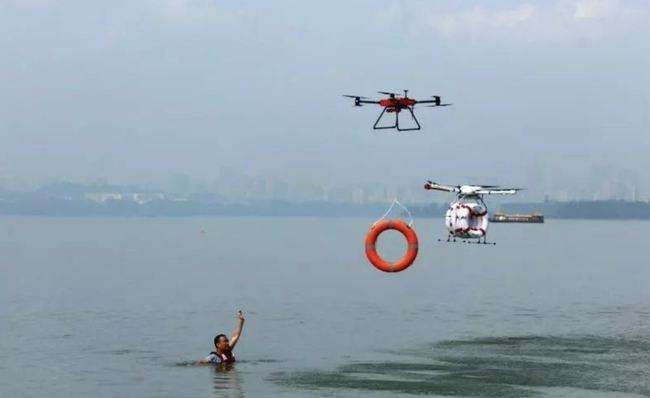
\includegraphics[width=12cm]{figures/fig_uvafun.png}
%     \caption{
%         无人机救援
%     }
%     \label{f1}
% \end{figure}
\begin{figure}[H]
    \vspace{12pt}  
    \centering
    \subfloat[运输]{
    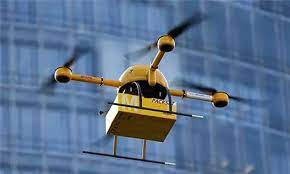
\includegraphics[width=6cm]{figures/fig_uvatransport.jpg}
    }
    \quad
    \subfloat[摄影]{
    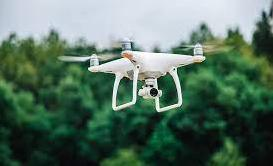
\includegraphics[width=6cm ]{figures/fig_uvashoot.jpg}
    }
    \quad
    \subfloat[监测]{
    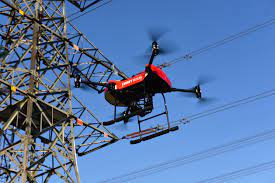
\includegraphics[width=6cm]{figures/fig_uvainspection.jpg}
    }
    \quad
    \subfloat[喷洒]{
    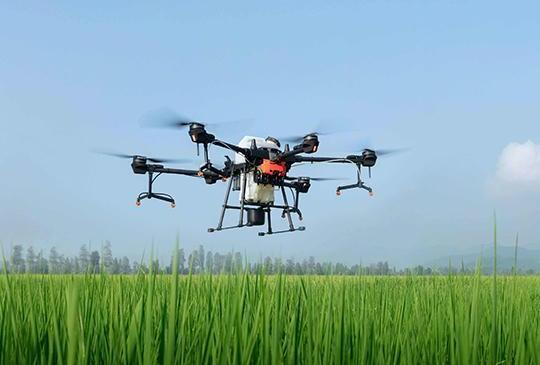
\includegraphics[width=6cm ]{figures/fig_uvafarm.jpg}
    }
    \caption{ 无人机应用}
    
\end{figure}


\section{研究现状}

随着无人机的应用领域越来越广泛,对于在一些高维、复杂和未知环境中飞行的无人机,安全变得至关重要。路径规划作为无人机飞行的关键技术,越来越受到研究者的重视。目前现有的适合无人机的路径搜索算法和路径优化方法大致如图 \ref{fig2} 所示。
\begin{figure}[H]
    \vspace{12pt}
    \centering
    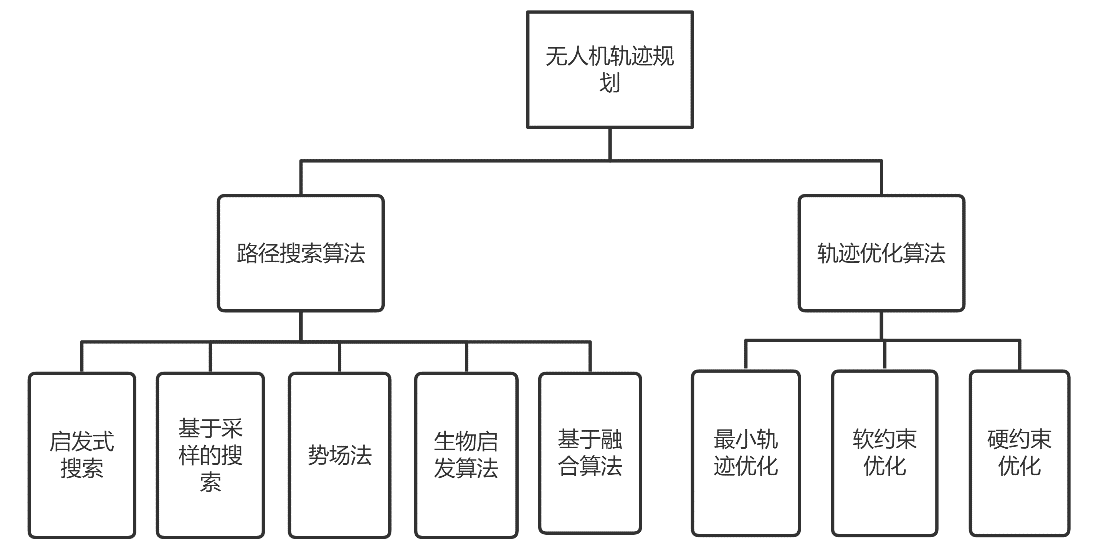
\includegraphics[width=12cm]{figures/fig2.png}
    \caption{
        常用算法
    }
    \label{fig2}
\end{figure}

\subsection{路径搜索算法}



\subsection{轨迹优化算法}


\section{本文研究内容}





\endinput

\chapter{轨迹规划的理论基础}
在进行轨迹规划之前,首先要明确轨迹规划的对象,已知无人机具有12维的状态参数,在做轨迹规划的过程中不可能对全维度空间进行规划,但是可以利用微分平坦理论证明只需对轨迹状态进行规划就可以达到控制无人机的目的,下面将对此进行证明。此外本章还介绍了后面章节会用到的贝塞尔曲线和优化问题,主要说明了曲线的基本特性和二次规划问题及其主要求解方式。

\section{无人机系统的微分平坦性}
微分平坦特性是系统本身的一种结构属性,一般地,对于一个控制系统来说,如果存在一组输出可以使得控制系统中的所有状态变量和控制输入变量都可以表示为这组输出及其有限阶微分的函数表达式,则认为此系统时微分平坦的。对于如式 \ref{equ_1} 所示的非线性系统:
\setlength\abovedisplayskip{0.15cm}
\setlength\belowdisplayskip{0.15cm}%公式
\begin{equation}
    \left\{ \begin{array}{l}
    \dot x = f(x,u),x \in {R^n},u \in {R^m}\\
    y = g(x),y \in {R^m}
    \end{array} 
    \right.
    \label{equ_1}
\end{equation}
其中$u$为输入,$y$为输出,$x$为系统状态变量,当系统存在输出${O = h(x,u,\dot u, \cdots ,{u^{(n - 1)}})}$使得:
\begin{equation}
    \begin{array}{l}
        x = x(O,\dot O, \cdots ,{O^{(n - 1)}})\\
        u = u(O,\dot O, \cdots ,{O^{(n - 1)}})
        \end{array}
        \label{equ_2}
\end{equation}
则称非线性系统是微分平坦的,此系统的微分平坦输出为${O}$。已知微分平坦输出${O}$的期望轨迹${O_d}$,就可以依据微分平坦的定义的到系统所有变量的期望表达式。

依据上述理论可以知道系统状态、输入和平坦输出与之间的关系是一一对应的,也就是所微分平坦系统的状态特性可由平坦输出唯一决定。同时,具有微分平坦特性的系统可以将状态变量$x$和控制输入$u$映射到平坦的输出空间中,而输出空间的维数总是低于状态空间$x$的维数,因此微分平坦理论常常用于轨迹规划问题。应用该理论可以将原本复杂的高维空间轨迹规划问题转化到低维的平坦空间处理,在该空间获得求解结果后通过一定的方式映射得到原状态空间的轨迹。此外,微分平坦特性还有个优点,它并不依赖于坐标系的选取,这同样也利于简化问题,便于轨迹规划。如果四旋翼无人机控制系统满足上述的微分平坦性,那么四旋翼无人机系统的输入量和状态栏都可以用此平坦输出及其微分表示。因此,下面将在理论方面对此进行论证\ucite{谈冰然2020基于空气动力学补偿的四旋翼无人机飞行控制与轨迹规划}。


\section{贝塞尔曲线}

贝塞尔曲线是一种以伯恩思坦多项式为基础的样条曲线,$n$阶贝塞尔曲线的多项式由$n+1$个线性无关的伯恩思坦基组成,并由$n+1$个控制点控制\ucite{sederberg2012computer}。


\endinput
\chapter{第三章标题}

\endinput
%\myemptypage
%\myemptypage
\chapter{第四章标题}

\endinput
%\myemptypage
%\myemptypage
\chapter{仿真实验与结果分析}
针对上述方法,对无人机轨迹规划方法进行仿真实验。首先在 MATLAB 上证明了优化策略的可行性,然后基于标准的无人机仿真框架搭建了仿真环境,设计了仿真流程,完成了 ROS、PX4、Gazebo 的联合仿真内容。
\section{MATLAB 平台}
\subsection{规划算法验证}
在MATLAB平台上验证路径搜索算法,在之前获得的速度场的基础上进行波形传播和速度搜索,图 \ref{fig_pathtimereal2} 为搜索出来的路径和到达时间图。

\begin{figure}[H]
    \centering
    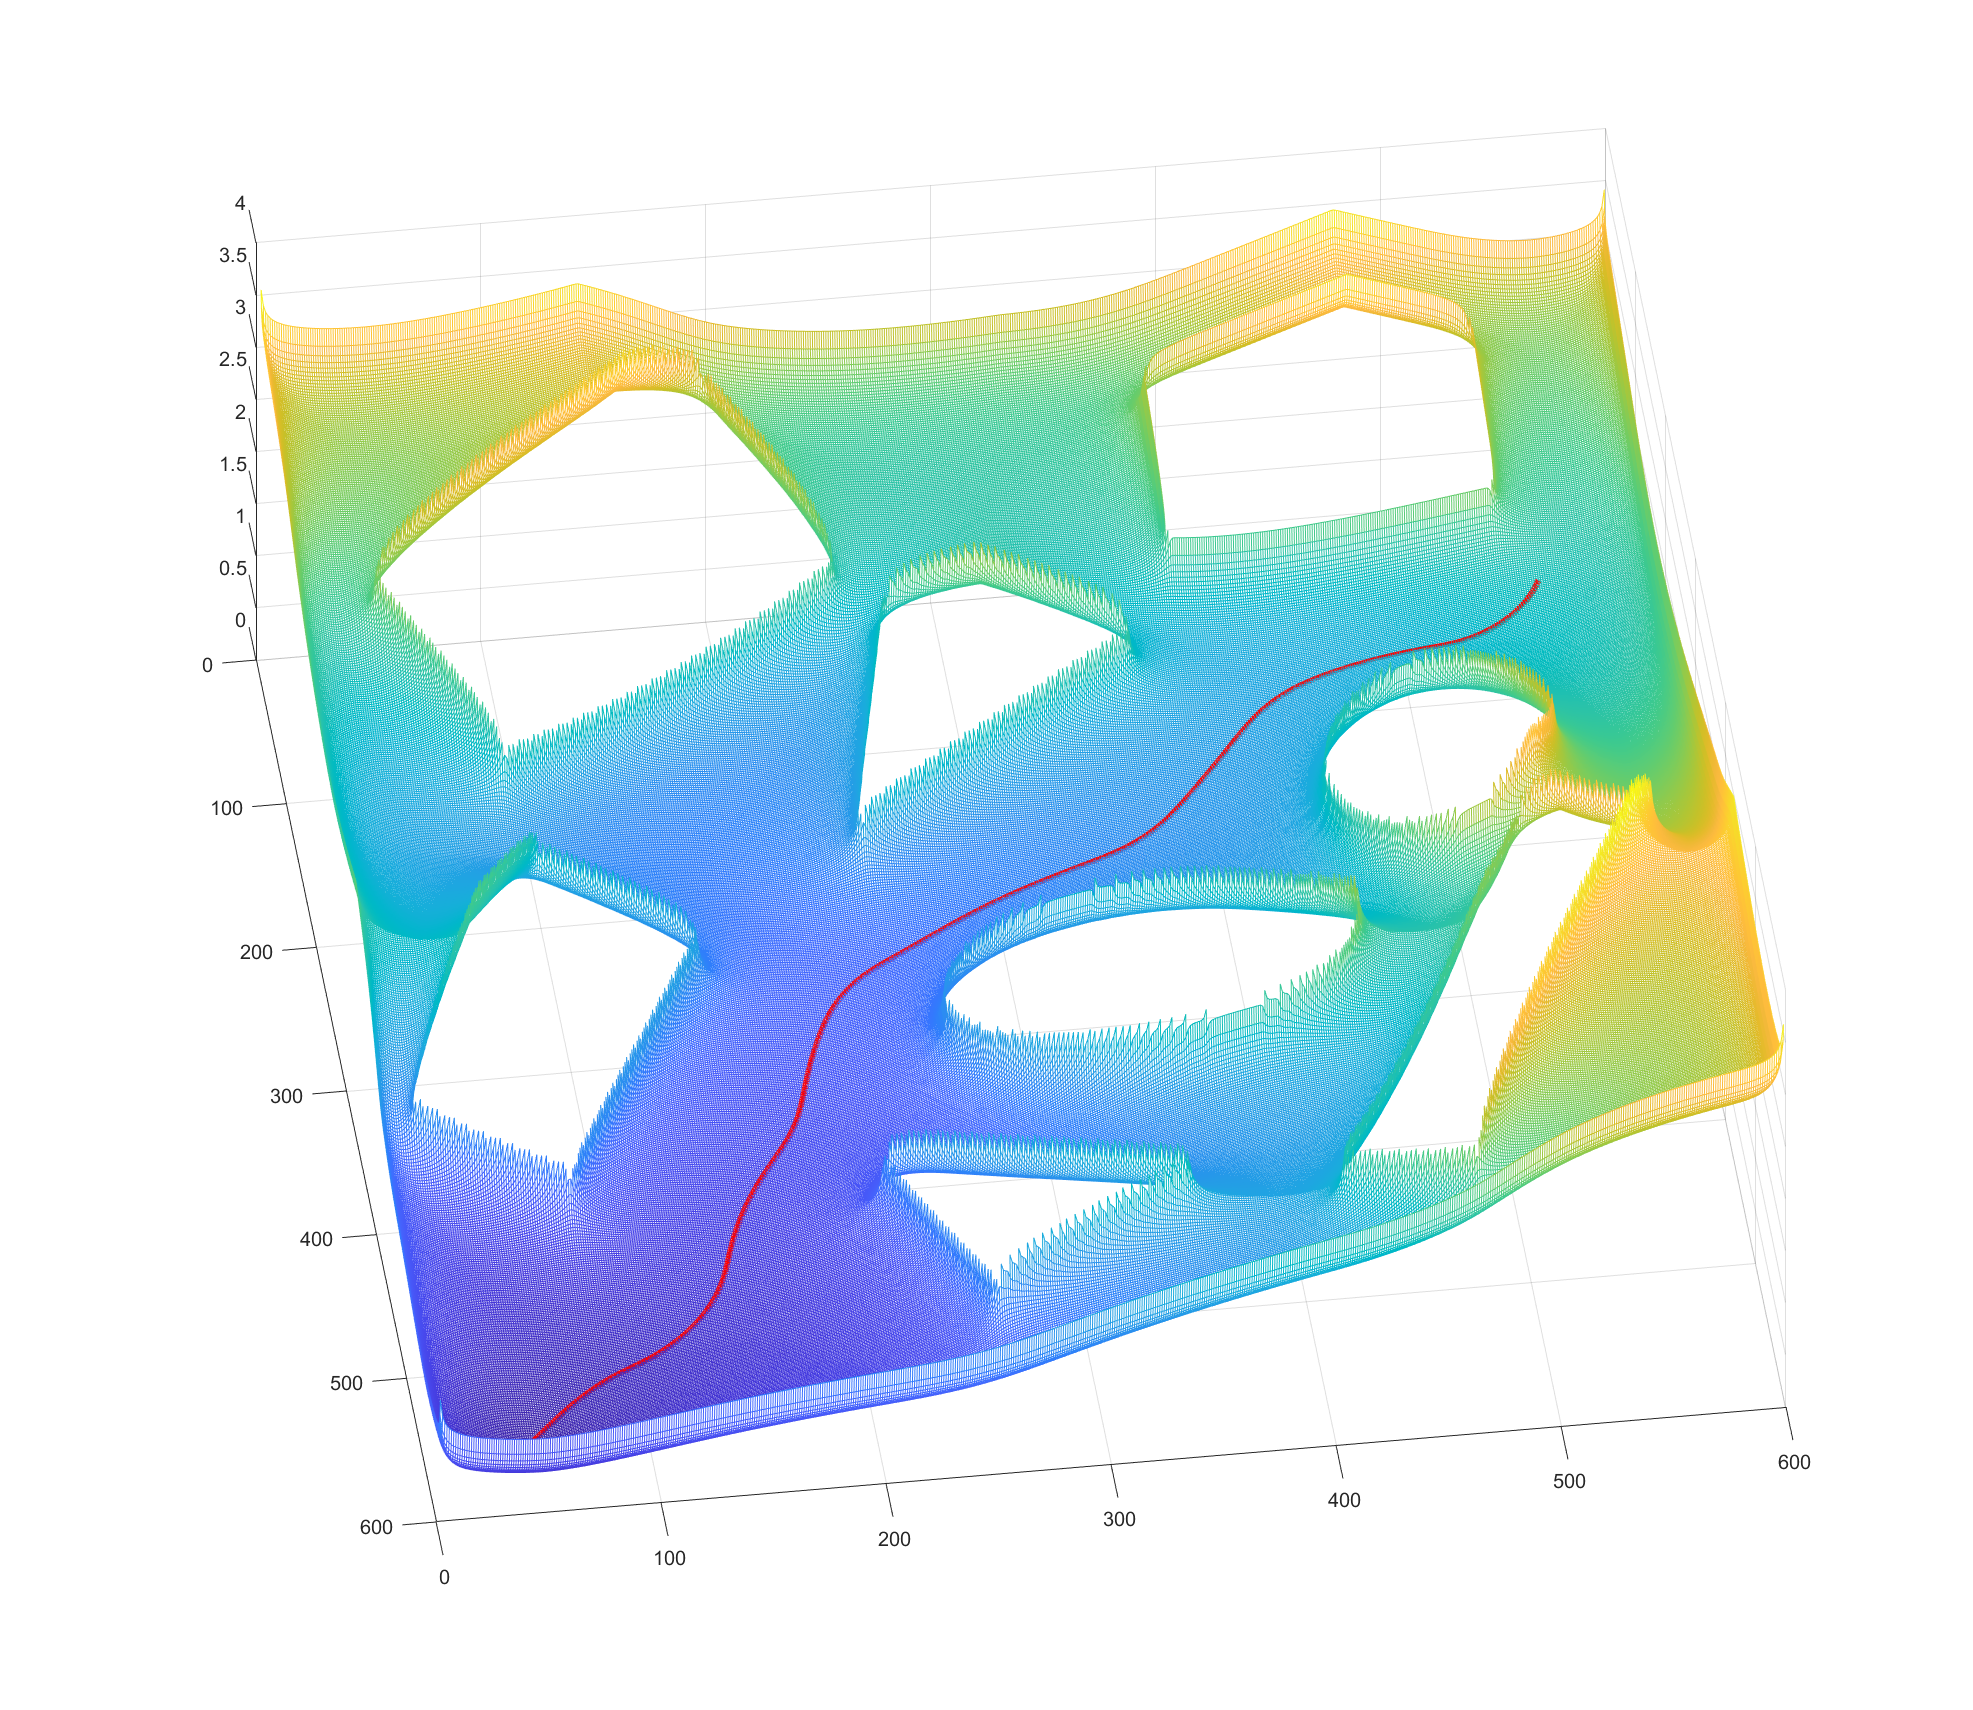
\includegraphics[width=12cm]{figures/fig_pathtimereal.png}
    \caption{
        路径和到达时间图
    }
    \label{fig_pathtimereal2}
\end{figure}

\begin{table}[H]
    \centering
    \caption{参数设置}
    \label{form_2}
    \begin{tabular}{cccccc}
    \hline
    \multirow{2}{*}{多项式阶数} & \multicolumn{2}{c}{最大速度限制} & \multicolumn{2}{c}{最大加速度限制} & \multirow{2}{*}{分段轨迹时间}       \\ \cline{2-5}
                           & x            & y           & x            & y            &                                                                                               \\ \hline
    5                      & 5m/s         & 5m/s        & 2 $m^2$/s       & 2 $m^2$/s       & \begin{tabular}[c]{@{}c@{}}{[}16.50;16.50;16.50;\\   16.50;16.50;16.50{]}(s)\end{tabular} \\ \hline
    \end{tabular}
\end{table}

表格可用https://www.tablesgenerator.com/ 在线工具转换
\endinput
\chapter{全文总结}
\section{总结}

\section{展望}


\endinput

% 参考文献设置
\clearpage
\phantomsection
% \chapter*{参考文献}
\addcontentsline{toc}{chapter}{\bf \fSong 参考文献}
% npu专用
\bibliographystyle{settings/nputhesis}
\renewcommand{\baselinestretch}{1.25}  
\setlength{\bibsep}{0.5ex} 
% 参考文献位置
\bibliography{references/reference}
% 附录
\backmatter
%\myemptypage
\renewcommand{\baselinestretch}{1.5}
\fontsize{12pt}{13pt}\selectfont
\phantomsection
\chapter*{致~~~谢}
\addcontentsline{toc}{chapter}{\bf \fSong 致~~~谢}

历时半年之久的毕业设计终于结束了。从最初的选题、写开题报告,到后来的编程、论文撰写,并不是一帆风顺的。在这期间,有很多人给我帮助,给我建议。




\clearpage
\endinput
%\myemptypage
\phantomsection
\chapter*{毕业设计小结}
\addcontentsline{toc}{chapter}{\bf \fSong 毕业设计小结}

毕业的日子即将到来,毕业设计也接近尾声。奋战了几个月,我的毕业设计终于完成了。。。。。

\clearpage
\endinput
% \phantomsection
\chapter*{附~~~录}
\addcontentsline{toc}{chapter}{\bf \fSong 附~~~录}


\clearpage
\endinput

\clearpage
\end{document}
